
% ----------------------------------------------------------------------
%  Set the document class
% ----------------------------------------------------------------------
\documentclass[11pt,a4paper,twoside]{article}

% ----------------------------------------------------------------------
% Define external packages, language, margins, fonts and new commands
% ----------------------------------------------------------------------
%\input{preamble} 
\usepackage[utf8]{inputenc}   % <<<<< Linux
\usepackage[english]{babel} % <<<<< English
\usepackage{notoccite}
\usepackage[skip=0.5\baselineskip]{caption}
\hyphenation{GTKWave}
\usepackage{listings}
\usepackage[all]{nowidow}

%blind text
\usepackage{lipsum}

\usepackage{graphicx}
\graphicspath{ {./} {../../figlib/} }
\def\FontLn{% 16 pt normal
  \usefont{T1}{phv}{m}{n}\fontsize{16pt}{16pt}\selectfont}
\def\FontLb{% 16 pt bold
  \usefont{T1}{phv}{b}{n}\fontsize{16pt}{16pt}\selectfont}
\def\FontMn{% 14 pt normal
  \usefont{T1}{phv}{m}{n}\fontsize{14pt}{14pt}\selectfont}
\def\FontMb{% 14 pt bold
  \usefont{T1}{phv}{b}{n}\fontsize{14pt}{14pt}\selectfont}
\def\FontSn{% 12 pt normal
  \usefont{T1}{phv}{m}{n}\fontsize{12pt}{12pt}\selectfont}

% Use Arial font as default
%
\renewcommand{\rmdefault}{phv}
\renewcommand{\sfdefault}{phv}
\usepackage{geometry}	
\geometry{verbose,tmargin=2.5cm,bmargin=2.5cm,lmargin=2.5cm,rmargin=2.5cm}

%\usepackage{setspace}
%\renewcommand{\baselinestretch}{1.5}

\usepackage[pdftex]{hyperref} % enhance documents that are to be
                              % output as HTML and PDF
\hypersetup{colorlinks,       % color text of links and anchors,
                              % eliminates borders around links
%            linkcolor=red,    % color for normal internal links
            linkcolor=black,  % color for normal internal links
            anchorcolor=black,% color for anchor text
%            citecolor=green,  % color for bibliographical citations
            citecolor=black,  % color for bibliographical citations
%            filecolor=magenta,% color for URLs which open local files
            filecolor=black,  % color for URLs which open local files
%            menucolor=red,    % color for Acrobat menu items
            menucolor=black,  % color for Acrobat menu items
%            pagecolor=red,    % color for links to other pages
            pagecolor=black,  % color for links to other pages
%            urlcolor=cyan,    % color for linked URLs
            urlcolor=black,   % color for linked URLs
	          bookmarks=true,         % create PDF bookmarks
	          bookmarksopen=false,    % don't expand bookmarks
	          bookmarksnumbered=true, % number bookmarks
	          pdftitle={report},
            pdfauthor={Andre C. Marta},
%            pdfsubject={Thesis Title},
%            pdfkeywords={Thesis Keywords},
            pdfstartview=FitV,
            pdfdisplaydoctitle=true}

\usepackage[numbers,sort&compress]{natbib} % <<<<< References in numbered list [1],[2],...
\usepackage{subcaption} 
\usepackage{mdframed}

%%%%%%%%%%%%%%%%%%%%%%%%%%%%%%%%%%%%%%%%%%%%%%%%%%%%%%%%%%%%%%%%%%%%%%%%
%     Begin Document                                                   %
%%%%%%%%%%%%%%%%%%%%%%%%%%%%%%%%%%%%%%%%%%%%%%%%%%%%%%%%%%%%%%%%%%%%%%%%


\begin{document}

% Set plain page style (no headers, footer with centered page number)
\pagestyle{plain}

% Set roman numbering (i,ii,...) before the start of chapters
%\pagenumbering{roman}

% ----------------------------------------------------------------------
%  Cover page
% ----------------------------------------------------------------------
%%%%%%%%%%%%%%%%%%%%%%%%%%%%%%%%%%%%%%%%%%%%%%%%%%%%%%%%%%%%%%%%%%%%%%%%
%                                                                      %
%     File: Thesis_FrontCover.tex                                      %
%     Tex Master: Thesis.tex                                           %
%                                                                      %
%     Author: Andre C. Marta                                           %
%     Last modified :  2 Jul 2015                                      %
%                                                                      %
%%%%%%%%%%%%%%%%%%%%%%%%%%%%%%%%%%%%%%%%%%%%%%%%%%%%%%%%%%%%%%%%%%%%%%%%

\thispagestyle {empty}

% IST Logo - Signature A
% parameters: bb=llx lly urx ury (bounding box), width=h_length, height=v_length, angle=angle, scale=factor, clip=true/false, draft=true/false. 
\includegraphics[bb=9.5cm 11cm 0cm 0cm,scale=0.29]{IST_A_CMYK_POS}

\begin{center}
%
% Figure (Image or plot)
\vspace{1.0cm}
% height = 50 mm
%\includegraphics[height=50mm]{Figures/Airbus_A350.jpg}

% Title, author and degree
\vspace{1cm}
{\FontLb Circuit Theory and Electronics Fundamentals 2020/2021} \\ % <<<<< EDIT TITLE
\vspace{1cm}
{\FontSn Integrated Masters in Aerospace Engineering, Técnico, University of Lisbon} \\ % <<<<< EDIT COURSE
\vspace{1cm}
{\FontSn First Laboratory Report} \\
\vspace{1cm}
{\FontSn March 25, 2021} \\ % <<<<< EDIT DATE (corresponds to date of oral examination)
%
\vspace{1cm}
{\FontSn Rui Rodrigues, 95844 \\ Tiago Silva, 95850\\ Tomás Ribeiro, 95854}

\end{center}



% ----------------------------------------------------------------------
% Dedication page (optional)
% ----------------------------------------------------------------------
%\input{dedication} 
%\cleardoublepage

% ----------------------------------------------------------------------
%  Acknowledgments (optional)
% ----------------------------------------------------------------------
%\input{acknowledgements}
%\cleardoublepage

% ----------------------------------------------------------------------
%  Abstract (both in English and Portuguese)
% ----------------------------------------------------------------------
%\input{resumo} 
%\cleardoublepage

%\input{abstract} 

% ----------------------------------------------------------------------
%  Table of contents, list of tables, list of figures and nomenclature
% ----------------------------------------------------------------------

% Table of contents
%
\tableofcontents

% List of tables
%\addcontentsline{toc}{section}{\listtablename}
%\listoftables
%\cleardoublepage 

% List of figures
%\addcontentsline{toc}{section}{\listfigurename}
%\listoffigures
%\cleardoublepage 

% Set arabic numbering (1,2,...) after preface
%
%\setcounter{page}{1}
%\pagenumbering{arabic}

% ----------------------------------------------------------------------
%  Body
% ----------------------------------------------------------------------

\section{Introduction}
\label{sec:introduction}

% state the learning objective
\paragraph{} 
The objective of this laboratory assignment is to 
The circuit can be seen in Figure~\ref{fig:circuit}.


\paragraph{}
In Section~\ref{sec:theoretical}, a theoretical introduction is made in order to contextualize all the main principles that sustain our analysis of the circuit. This circuit is carefully analysed in Section~\ref{sec:analysis}, where the results are obtained in GNU Octave. Also, in Section~\ref{sec:simulation}, the circuit is analysed by simulation through the use of NGSpice to simulate the electric circuit behaviour. The results of the simulation of Section~\ref{sec:simulation} are then compared to the theoretical results obtained in Section~\ref{sec:analysis} and the comparative results are expressed in Section~\ref{sec:erroranalysis}. The conclusions of this study are outlined in the final part of the report, in Section~\ref{sec:conclusion}.


\begin{figure}[h] \centering
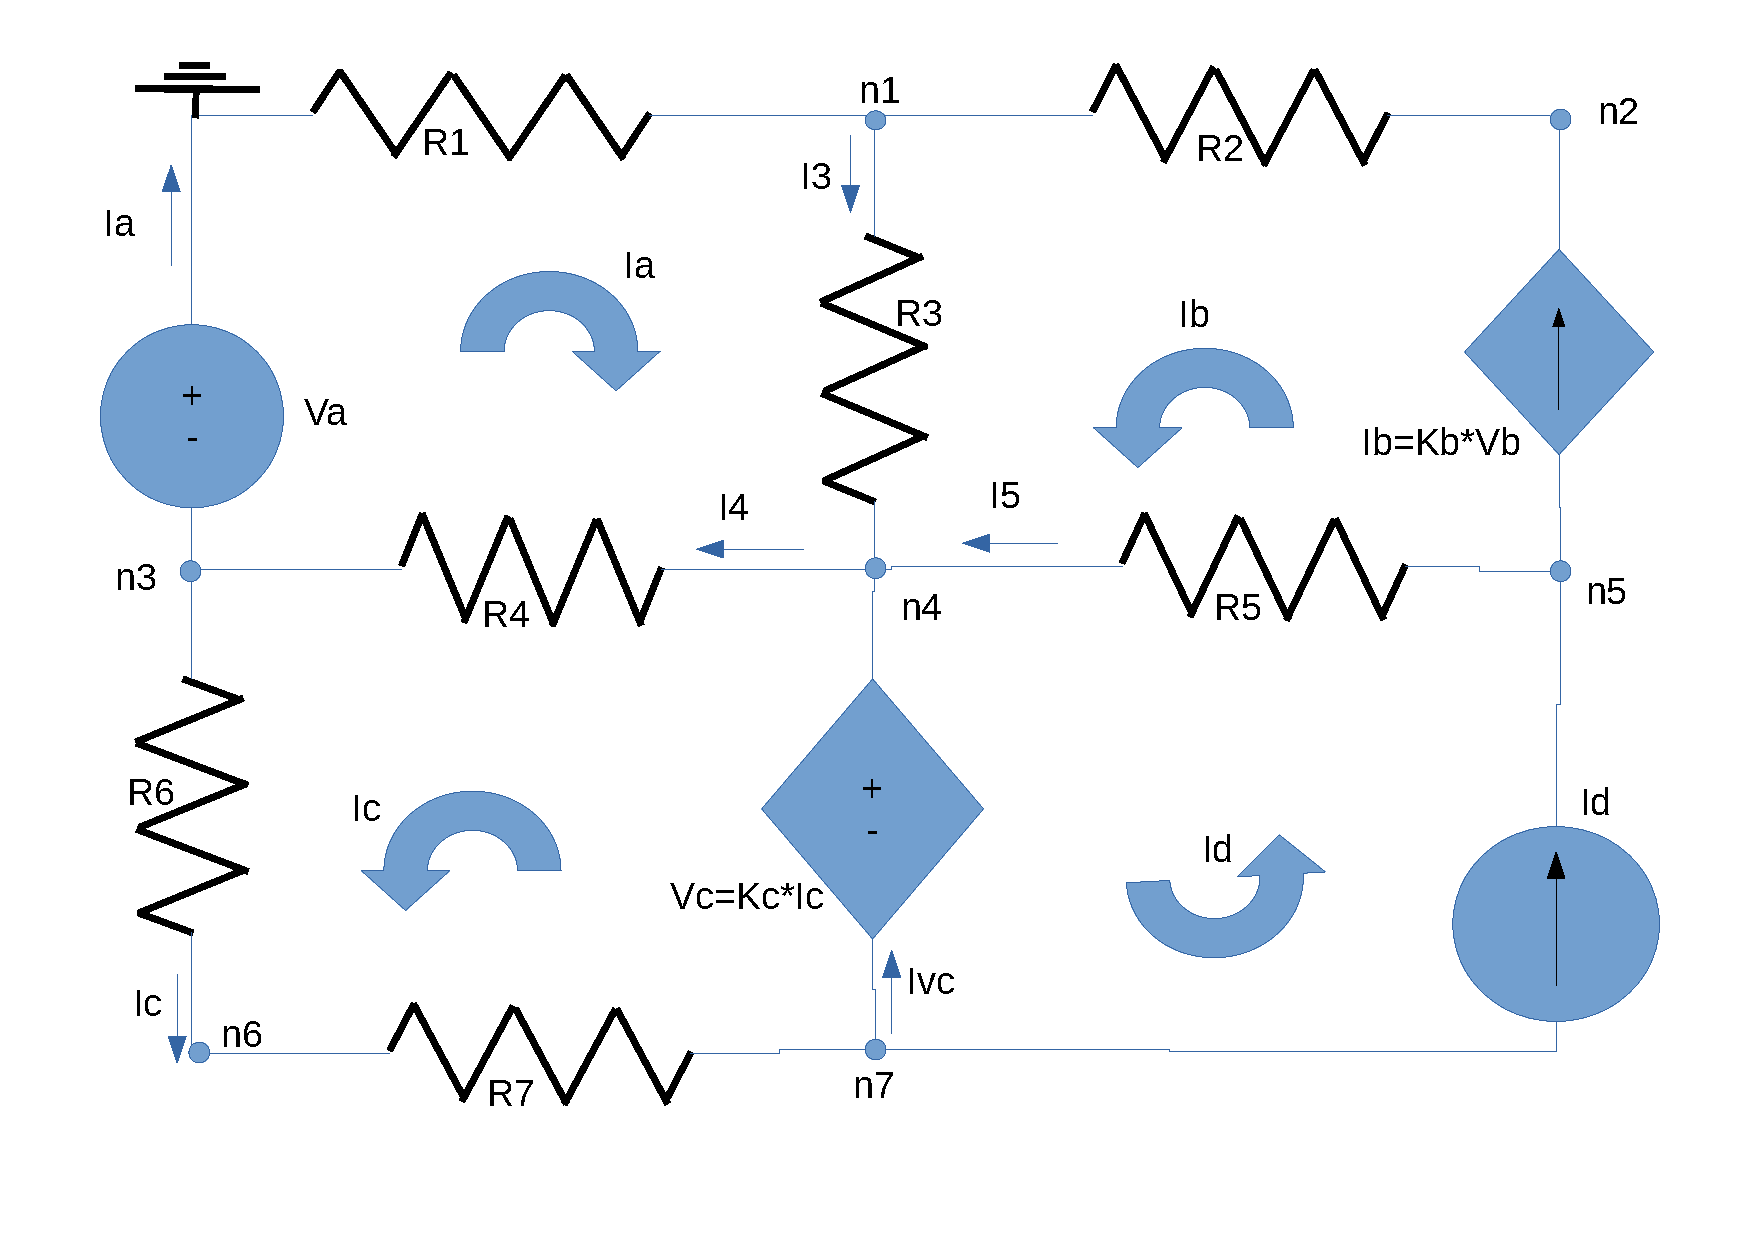
\includegraphics[width=0.4\linewidth]{circuit.pdf}
\caption{Third laboratory circuit.}
\label{fig:circuit}
\end{figure}



\section{Theoretical Analysis}
\label{sec:analysis}

\paragraph{}
%In this section, we can find the results of each topic required in the theoretical analysis. The numeric results or graphics are presented alongside a short explanation of the interpretation of the problem. All of the results were obatined usig GNU octave and the section is dividid in six different subsections - Subsection ~\ref{subsec:first_topic}, Subsection ~\ref{subsec:second_topic}, Subsection ~\ref{subsec:third_topic}, Subsection ~\ref{subsec:fourth_topic}, Subsection ~\ref{subsec:fifth_topic} and Subsection ~\ref{subsec:sixth_topic} -, one for each topic of the theoretical analysis.

\subsection{Theoretical - Topic I}
\label{subsec:first_topic}

\begin{center}
   \begin{tabular}{|c||c|}
      \hline    
      \multicolumn{2}{|c|} {\bf } \\
      \hline
        \input{}
   \end{tabular}
 \end{center}

 %%%%%%%%%%%%%%%%%%%%%%%%%%%%%%%%%

\subsection{Theoretical - Topic II}
\label{subsec:second_topic}


\begin{center}
   \begin{tabular}{|c||c|}
      \hline    
      \multicolumn{2}{|c|} {\bf } \\
      \hline
        \input{}
   \end{tabular}
 \end{center}
 

 %%%%%%%%%%%%%%%%%%%%%%%%%%%%%%%%%
 
\subsection{Theoretical - Topic III}
\label{subsec:third_topic}

\begin{figure}[H] \centering
\includegraphics[width=0.6\textwidth]{}
\caption{}
\label{}
\end{figure}



 %%%%%%%%%%%%%%%%%%%%%%%%%%%%%%%%%
 
\subsection{Theoretical - Topic IV}
\label{subsec:fourth_topic}

\paragraph{}
The forced response is where the output (the voltage on the capacitor) is going to end up in the long run after all stored energy eventually dissipates. This occors by ignoring the presence of energy storage elements (in our circuit analysis, it ignores the capacitor and its initial voltage, $V_x$). As suggested, plotting the amplitude and phase shift of a sinusoid in a complex plane, we get a complex number in polar form that we can apply to the circuit analysis: a phasor voltage source, $V_s$ = 1. Besides that, we also replaced $C$ with its impedance $Z_C=\frac{1}{\omega C}$.


\[
\left\{\begin{matrix}
f = 1 kHz = 1000 Hz \\
t = 20 ms = 0.020 s \\
\end{matrix}\right.
\]


\begin{center}
   \begin{tabular}{|c||c|}
      \hline    
      \multicolumn{2}{|c|} {\bf Nodal Analysis of Phasors [in Volts]} \\
      \hline
        
 Phasor of Node 1 & 6.12323399574e-17+i1.57079632679e+00 \\ \hline 
 Phasor of Node 2 & 5.78536935465e-17+i1.57079632679e+00 \\ \hline 
 Phasor of Node 3 & 5.10414916043e-17+i1.57079632679e+00 \\ \hline 
 Phasor of Node 5 & 5.83210704339e-17+i1.57079632679e+00 \\ \hline 
 Phasor of Node 6 & 8.26523333807e-02+i-1.42082340747e+00 \\ \hline 
 Phasor of Node 7 & -2.29152014669e-17+i-1.57079632679e+00 \\ \hline 
 Phasor of Node 8 & -3.40788140178e-17+i-1.57079632679e+00 \\ \hline 
   \end{tabular}
 \end{center}
  %%%%%%%%%%%%%%%%%%%%%%%%%%%%%%%%%
 
\subsection{Theoretical - Topic V}
\label{subsec:fifth_topic}

\paragraph{}
The natural response considers the internal initial conditions. The forced response considers the external inputs. Given that, we get the total response by summing the two responses, natural and forced. In fact, this is the principle of superposition in action (in the mathematical sense of differential equations).

\[
\left\{\begin{matrix}
v_t=v_n+v_f\\
f = 1 kHz = 1000 Hz \\
\end{matrix}\right.
\]

\begin{figure}[H] \centering
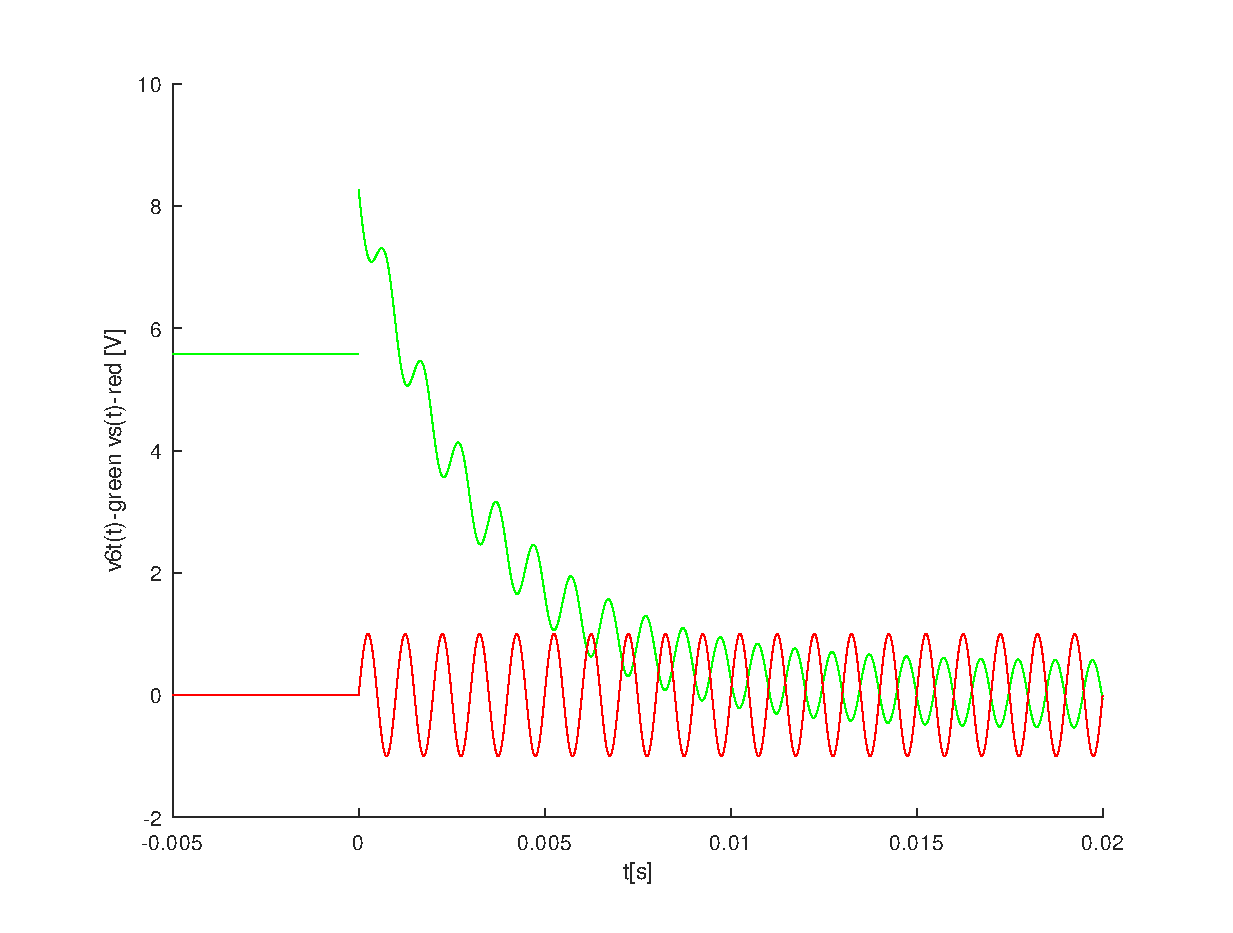
\includegraphics[width=0.6\textwidth]{total.eps}
\caption{The final total solution, $V6(t)$,  and $v_s(t)$ during time interval [-5, 20] ms.}
\label{fig:theo_fifth}
\end{figure}


Where $t$ is expressed in seconds (s) along the x-axis and 
$V6(t)$, the total solution, and $v_s$ are expressed in Volts (V) along the y-axis.

In the graphic above, it is ineteresting to note that, while the voltage emited by the source $V_s$ is constant, the node 6 will also have a constant voltage. This is because for $t<0$ the circuit will essentially behave as one of continuos current. After this time mark, the circuit reveals its alternate current nature and both the voltages of the source and of node 6 will vary sinousoidally.



  
  %%%%%%%%%%%%%%%%%%%%%%%%%%%%%%%%%

\subsection{Theoretical - Topic VI}
\label{subsec:sixth_topic}

\paragraph{}In this subsection, an analysis of the variation of the magnitude and phase of the phasors of $V_c$ $V_6$ and $V_s$ is made in function of the frequency. The first graphic presents the study of the variation of the magnitude and the second the study of the fase. In both graphics, the frequency $f$ in the x-axis varies from 0.1Hz to 1MHz


\[
\left\{\begin{matrix}
f =\in [0.1 , 1] MHz \\
v_c(f)=v_6(f)-v_8(f) \\
\end{matrix}\right.
\]


\begin{figure}[H] \centering
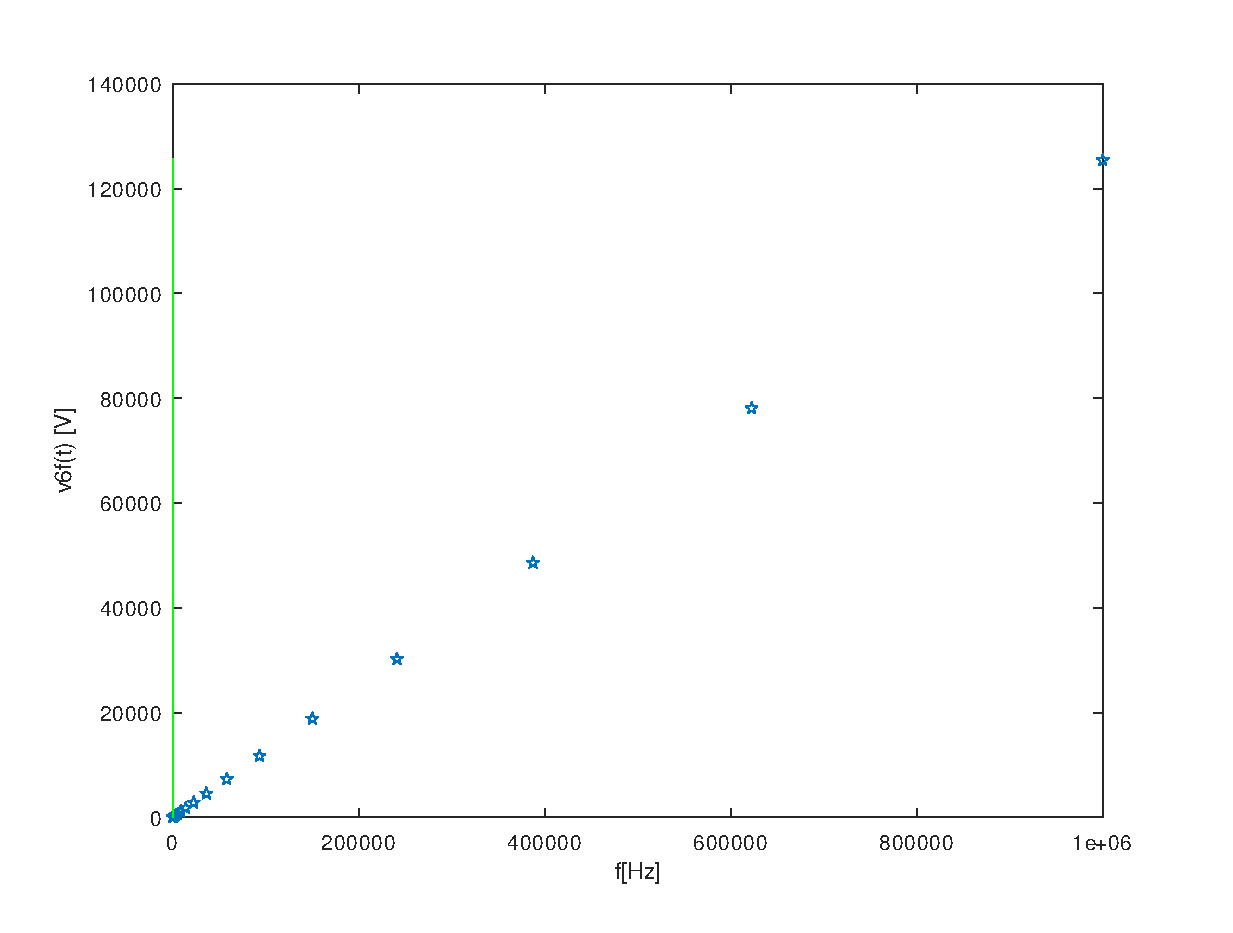
\includegraphics[width=0.6\textwidth]{magnitude.eps}
\caption{Magnitude of $v_s(f)$,  $v_c(f)$  and $v_6(f)$ during frequency interval [0.1 , 1] MHz.}
\label{fig:magnitudetheo}
\end{figure}

The frequency $f$ is expressed in Hertz (Hz) along the x-axis and 
the magnitude of $v_s(f)$,  $v_c(f)$  and $v_6(f)$ is expressed with a logscale decibel (dB) along the y-axis.\\ \\
When looking at this graph, a couple of things are important to highlight. First, $V_s$ will always have magnitude 0 because, given that its absolute value is 1 and we are using a logscale, $log(1)=0$. Second, we also note that the $v_c$ graph line does not resemble the one that represents $v_6$. This is because the voltage of the node 8 will also vary. 


\begin{figure}[H] \centering
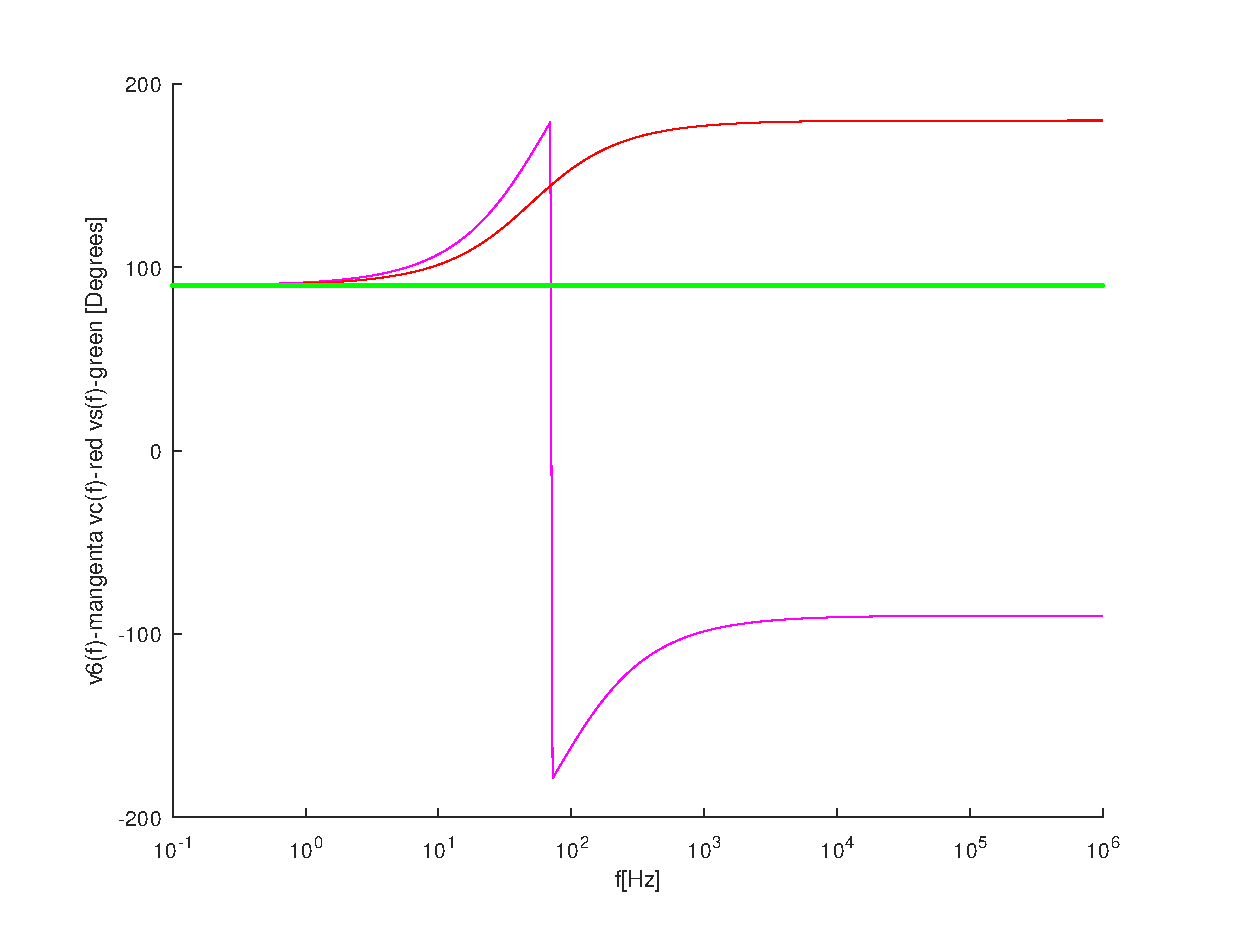
\includegraphics[width=0.6\textwidth]{phase.eps}
\caption{Phase $v_s(f)$,  $v_c(f)$  and $v_6(f)$ during frequency interval [0.1 , 1] MHz.}
\label{fig:phasetheo}
\end{figure}

The frequency $f$ is expressed in Hertz (Hz) along the x-axis and
the phase of $v_s(f)$,  $v_c(f)$  and $v_6(f)$ is expressed in degrees along the y-axis.\\ \\
In this graph, the first thing that comes to the eye is the fact that the phase of $V_s$ will always be constant and that, once again, the $v_c$ graph line does not resemble the one that represents $v_6$. 



\section{Simulation Analysis}
\label{sec:simulation}

In this section, we can find the results of each topic required in the simulation analysis. The numeric results or graphics are presented alongside a short explanation of the interpretation of the problem. All of the results were obtained using NGSpice and the section is divided in two different subsections. 

In this part of the lab, we tried to build the circuit in such a way that it would be as similar as possible as the one used in the Octave theoretical part. The most important difference between both approaches is that in Ngspice we had to use more diodes in the regulator circuit than in Octave. This is because while in Octave we used the standard diode voltage ($0.7 V$), requiring 17 diodes, in Ngspice that wasn't possible because diodes have varying voltages. Given that, our Ngspice voltage regulator circuit is made of 23 diodes.

Another difference from the Octave model, is that the ideal diode model used in the envelope circuit is not possible to replicate in Ngspice. However, this does not affect the final results because the transformer conversion factor was updated to compensate the fact that there is going to be a voltage drop in the envelope circuit diodes.

\subsection{Envelope Circuit Output}


For this envelope circuit we used the following values:
\[
\left\{\begin{matrix}
f = 50 Hz\\
n=13.5304 V\\
R=50k\Omega\\
C=150 \mu F
\end{matrix}\right.
\]

\begin{figure}[H] \centering
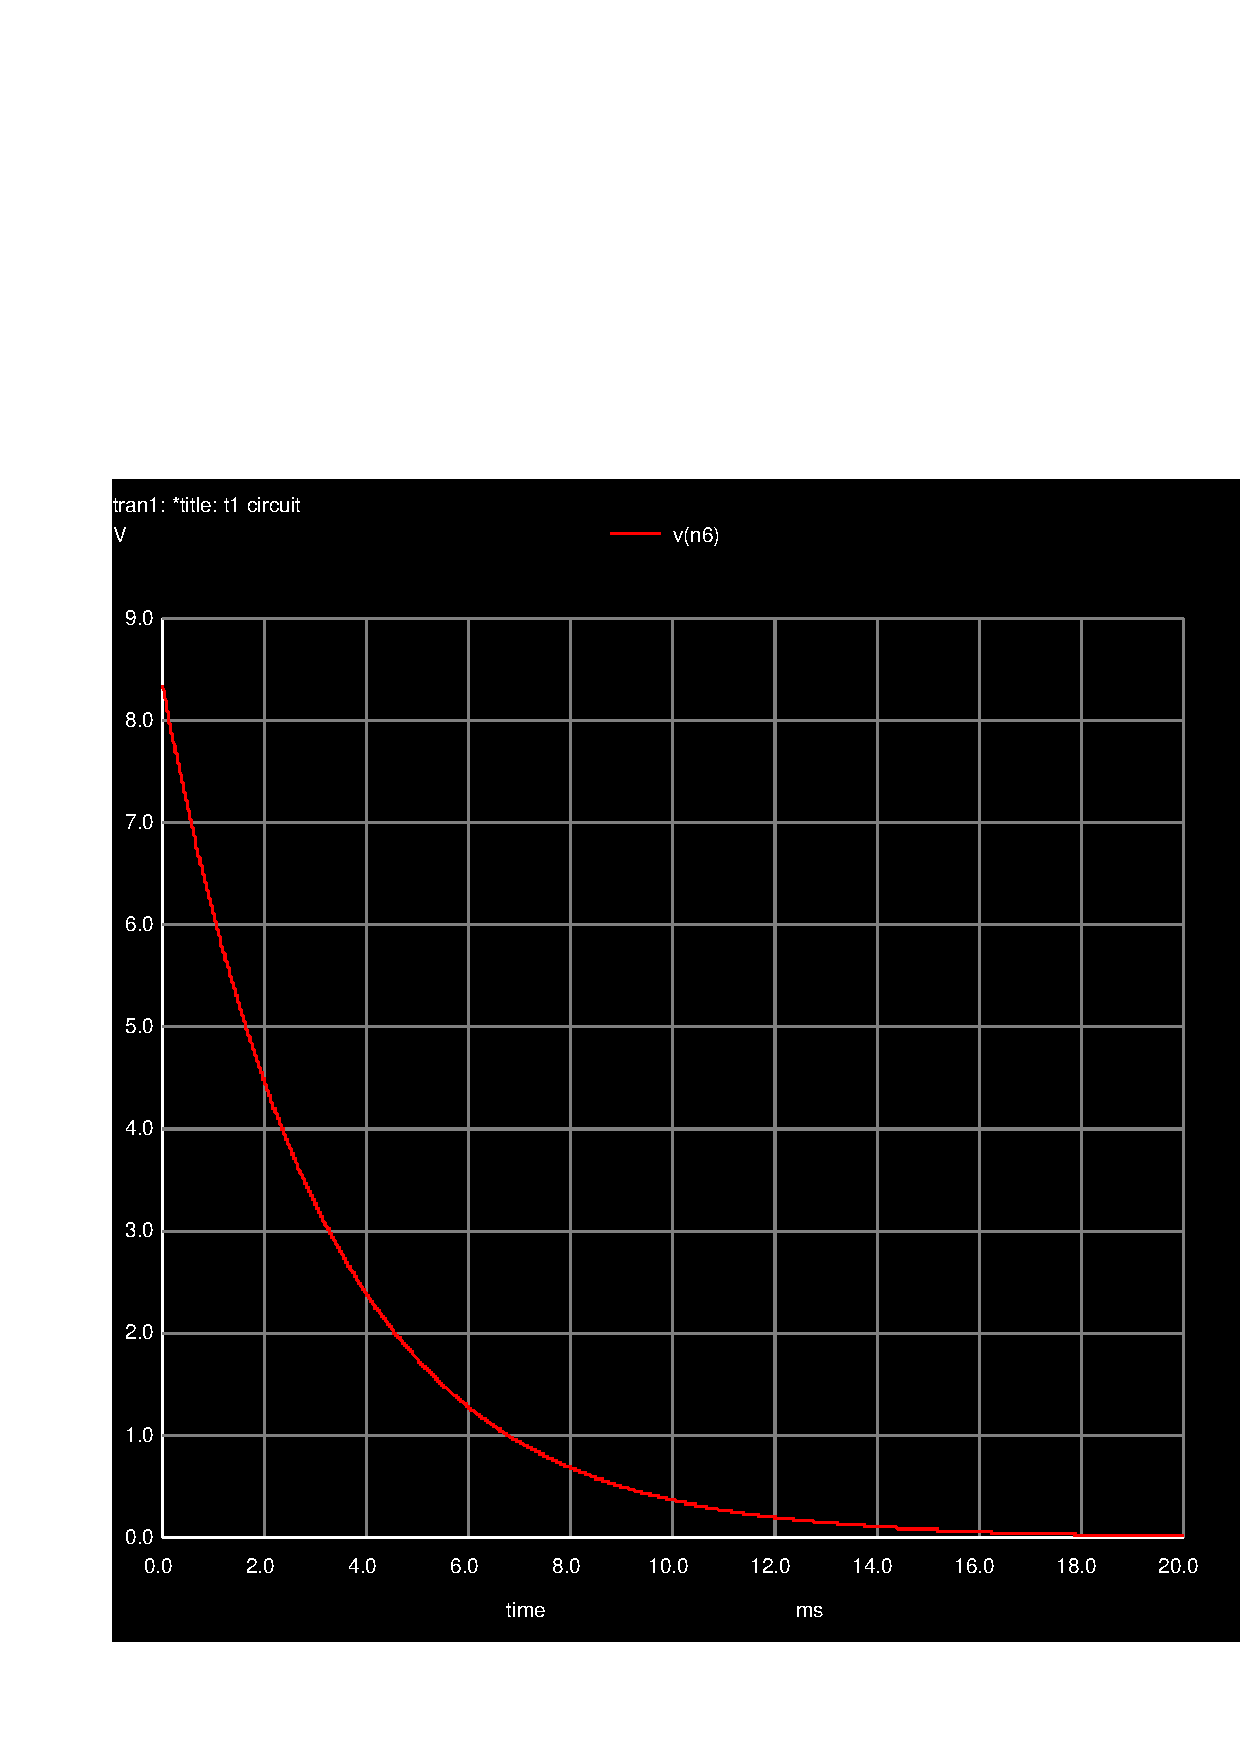
\includegraphics[trim= 0cm 0cm 0cm 10cm, clip, width=0.7\textwidth]{trans1.pdf}
\caption{The final envelope detector circuit voltage $v_0$ during 10 periods}
\label{fig:sim_envelope}
\end{figure}


In the graphic above, it is possible to see that, even though it is not the final result of the whole converter, it is already very close to $12V$. It is important to note that, if we zoom in, there will be a certain level of ripple that may affect our desired result, given that the signal hasn't gone throught the voltage regulator yet. Still on this topic, a particularity of Ngspice is the rising line at the very beginning which clearly stands for some transient the software uses.

\subsection{Circuit Output}


In this part the total output of the circuit is analysed.
The voltage regulator had its resistor set with a value of $10 Ohms$ and a total number of 23 diodes.

\begin{figure}[H]\centering
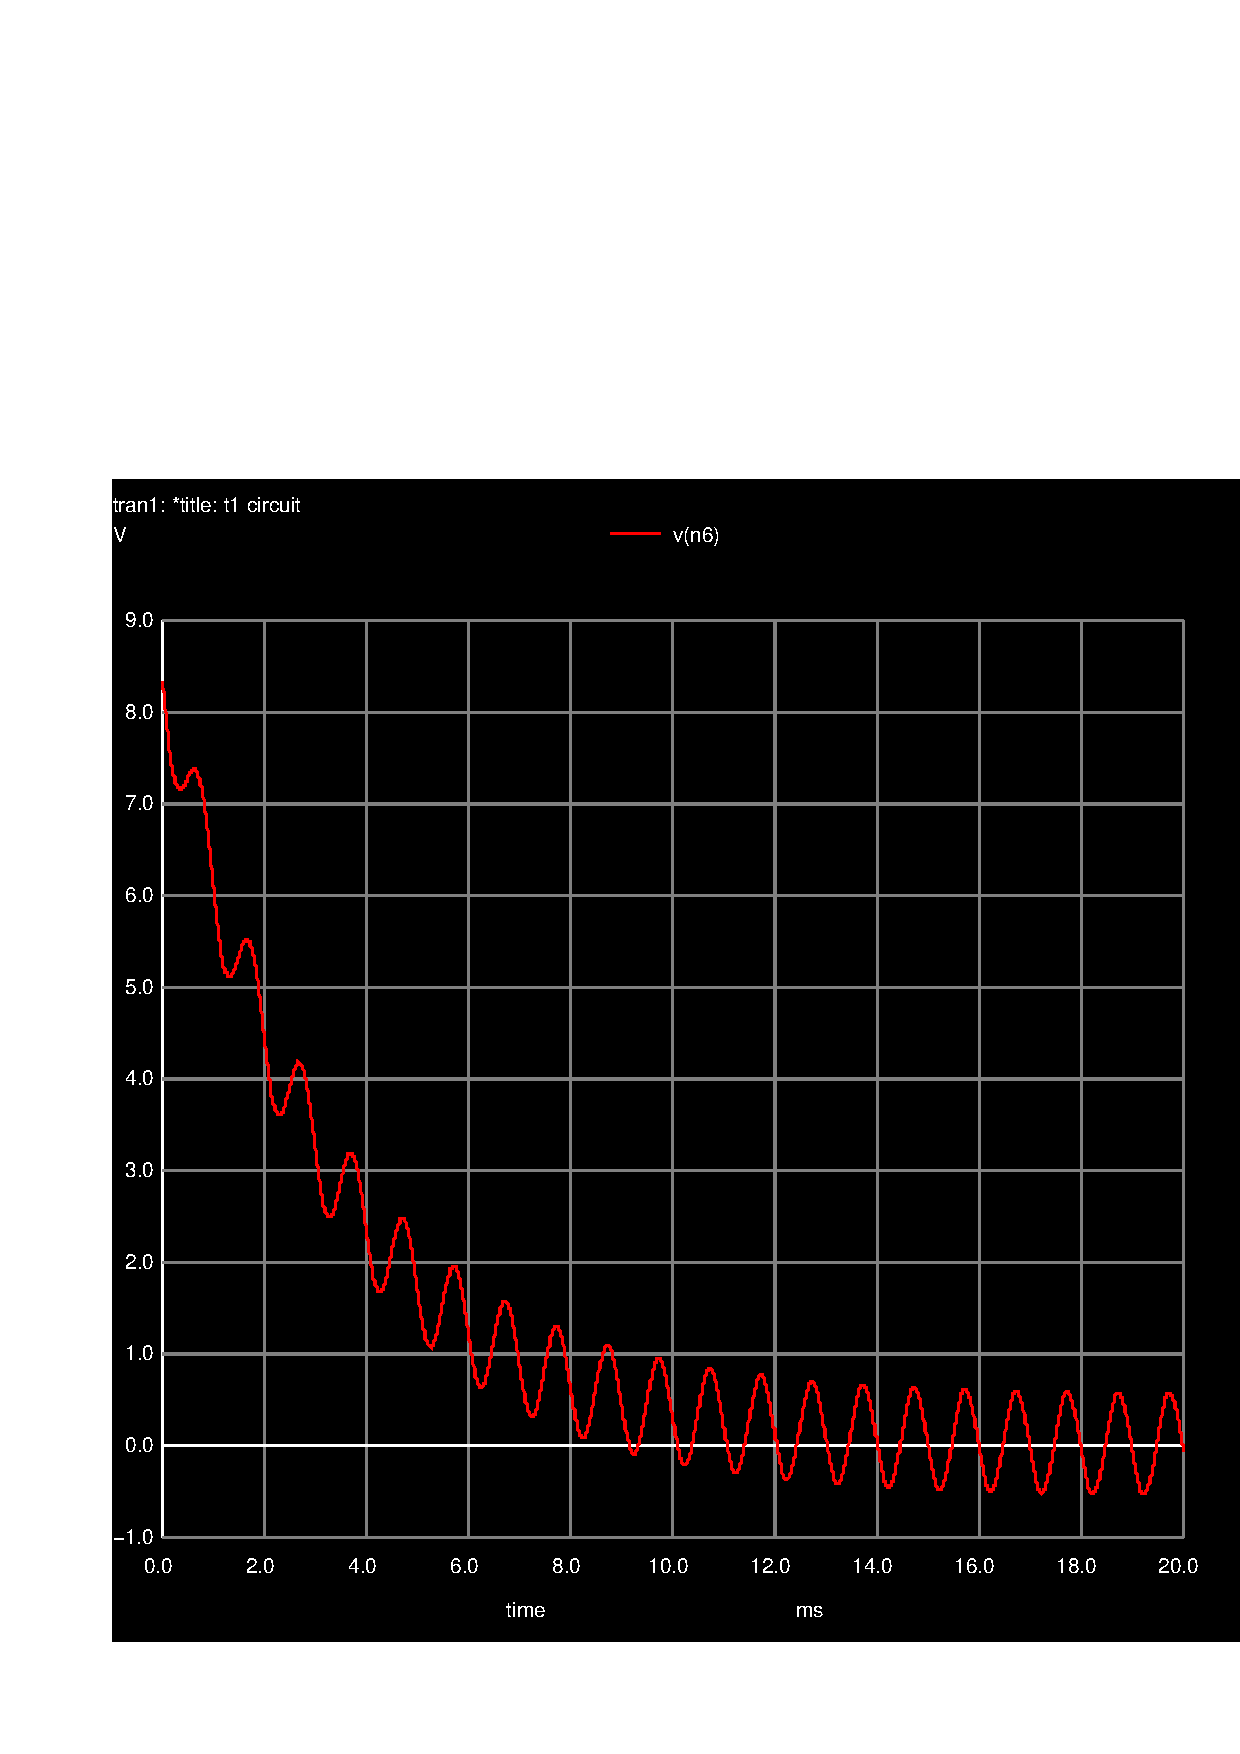
\includegraphics[trim= 0cm 0cm 0cm 10cm, clip, width=0.7\textwidth]{trans2.pdf}
\caption{The final output voltage $v_0$ during 10 periods}
\label{fig:sim_output}
\end{figure}

In the graphic above, the output voltage is represented. Looking at it is enough to understand that the final voltage is very close to the desired $12V$, however the difference that remains will be discussed below.

\begin{figure}[H]\centering
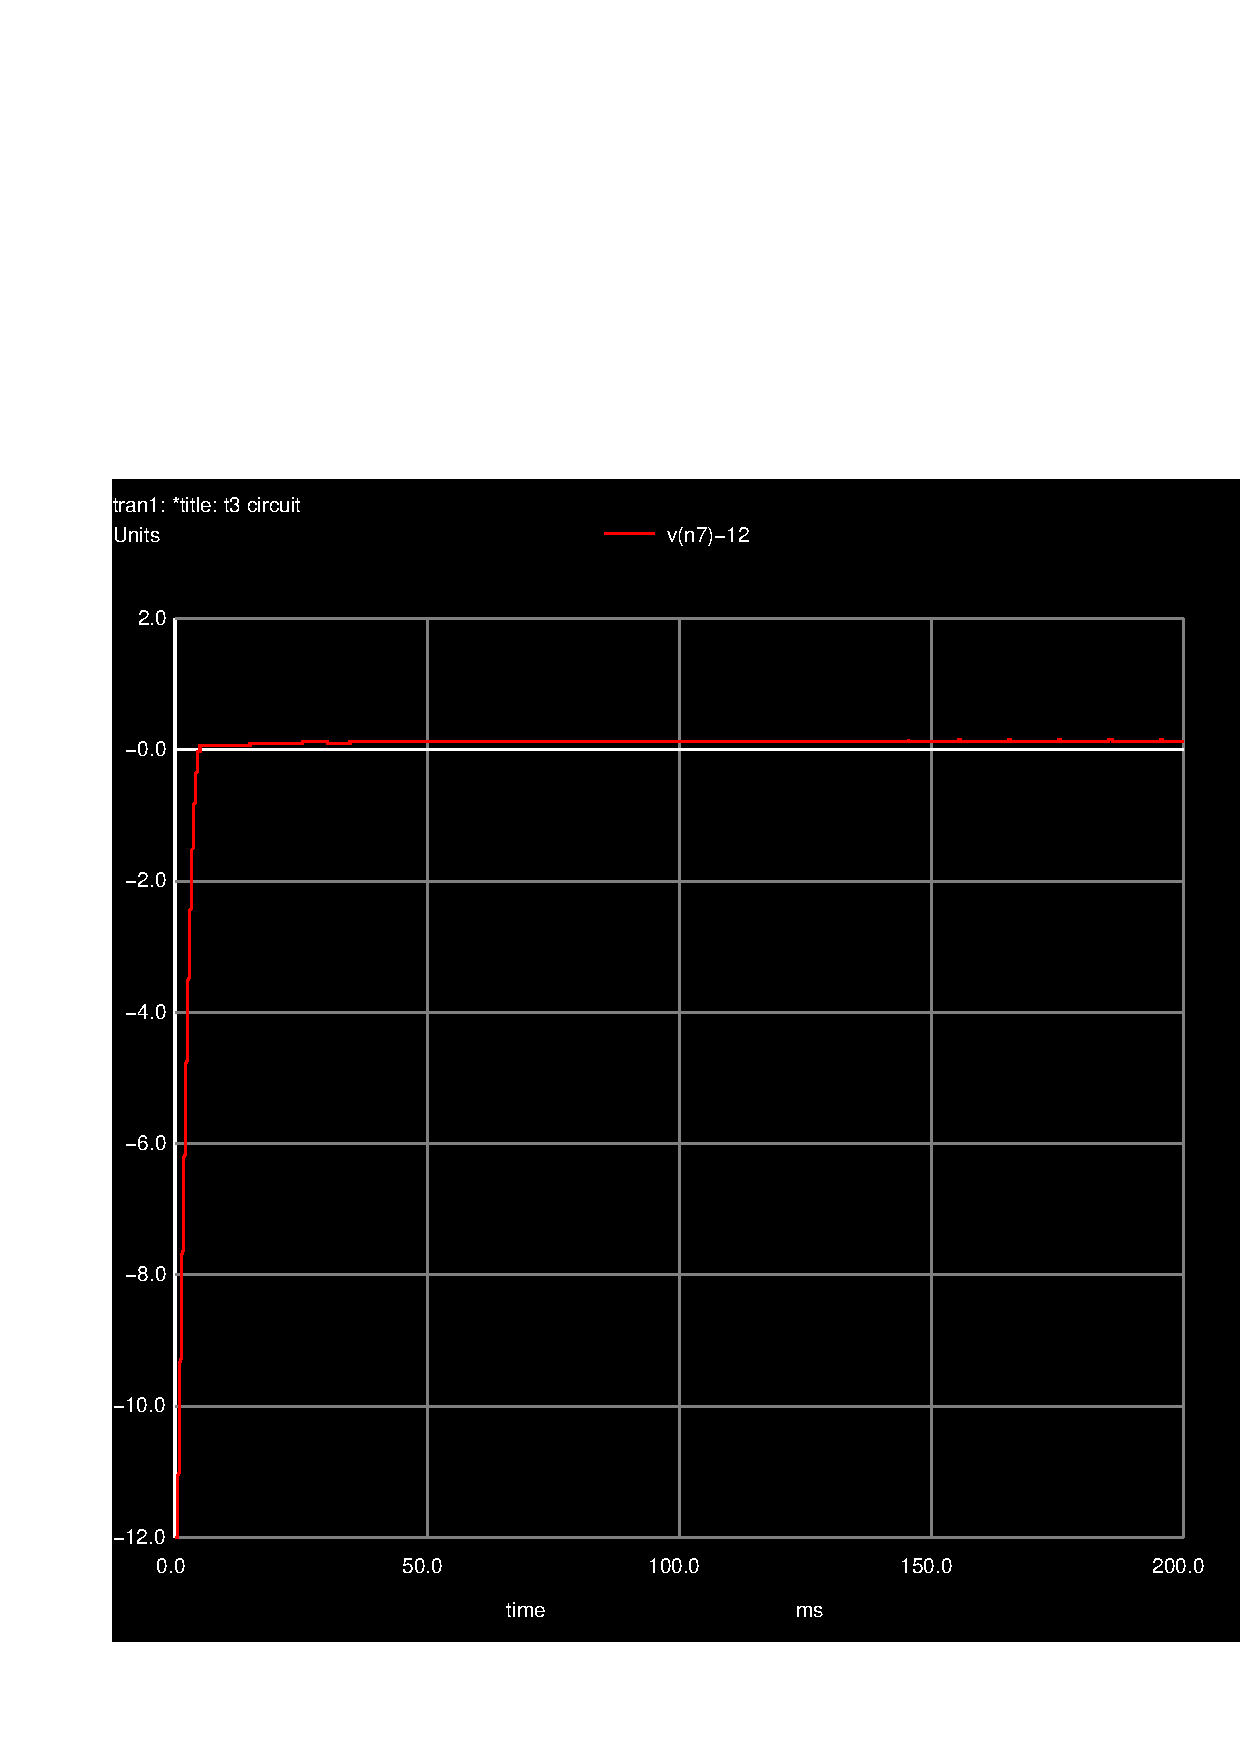
\includegraphics[trim= 0cm 0cm 0cm 10cm, clip, width=0.7\textwidth]{trans3.pdf}
\caption{The final output voltage $v_0$ subtracted by 12 during 10 periods}
\label{fig:sim_outputdiff}
\end{figure}

The graphic above essentialy shows the ripple of the circuit, which is basically how much the output voltage deviates from $12V$ and, once again, the results are pretty satisfying, with the line being very close to zero for most of the 10 periods. Still, below we can find a table with more accurate ripple data at a numerical level, which will confirm the theory that the simulation was well-succeeded.


\begin{table}[H] \centering
  \begin{tabular}{|l|r|}
    \hline    
    {\bf Data} & {\bf Value} \\ \hline
    \input{op_TAB}
  \end{tabular}
  \caption{}
 \label{tab:op}
\end{table}

From the table above, we can see that the average has a pretty good result being pratically $12V$. When it comes to the ripple, it also has a very good result, with an order of significance in the hundredths.


\section{Conclusion}
\label{sec:conclusion}



%\cleardoublepage

% ----------------------------------------------------------------------
%  Bibliography
% ----------------------------------------------------------------------
%\addcontentsline{toc}{section}{\bibname}
%\bibliographystyle{abbrvunsrtnat} % <<<<< SELECT IF USING REFERENCES BY NUMBER (CITATION ORDER)
%\bibliography{../../../BIBfile.bib}

% ----------------------------------------------------------------------
\end{document}
% ----------------------------------------------------------------------

